\documentclass[dvips,landscape]{foils}
\usepackage{graphicx,psfrag}
\usepackage{graphics}
\usepackage{amsmath}
\usepackage{amsthm}
\usepackage{amsfonts}
\input defs.tex
\raggedright
\special{! TeXDict begin /landplus90{true}store end }
\renewcommand{\oursection}[1]{
\foilhead[-1.0cm]{#1}
}

\title{Topology Optimization in Microfluidic Mixing Channel and Cutoff Phenomenon in Chaotic Mixing}
\author{Tzu-Chen Liang}
\MyLogo{Tzu-Chen Liang, Stanford University}
\date{\today}
\newtheorem{definition}{Definition}
\newtheorem{example}{Example}
\newtheorem{theorem}{Theorem}
\newtheorem{lemma}{Lemma}


% Here are the 3 topics
\newcommand{\mytopica}{Topology optimization of microfluidic mixing problems}
\newcommand{\mytopicb}{Numerical evidences of cutoff phenomena in chaotic mixing}
\newcommand{\mytopicc}{Symbolic dynamics and cutoff phenomenon }


\begin{document}
%\setlength{\parskip}{0cm}
\maketitle
%%%%%%%%%%%%%%%%%%%%%%%%%%%%%%%%%%%%%%%%%%%%%%%%%%%%%%%%%%%%%%%%%%%%%%%%
\newpage
\oursection{Outline}
\begin{itemize}
\item \mytopica 
\item \mytopicb 
\item \mytopicc 
\end{itemize}
%%%%%%%%%%%%%%%%%%%%%%%%%%%%%%%%%%%%%%%%%%%%%%%%%%%%%%%%%%%%%%%%%%%%%%%%%
%%%%%%%%%%%%%%%%%%%%%%%%%%%%%%%%%%%%%%%%%%%%%%%%%%%%%%%%%%%%%%%%%%%%%%%%%
%%%%%%%%%%%%%                 TOPIC a                          %%%%%%%%%%
%%%%%%%%%%%%%%%%%%%%%%%%%%%%%%%%%%%%%%%%%%%%%%%%%%%%%%%%%%%%%%%%%%%%%%%%%
%%%%%%%%%%%%%%%%%%%%%%%%%%%%%%%%%%%%%%%%%%%%%%%%%%%%%%%%%%%%%%%%%%%%%%%%%
\newpage
\oursection{\mytopica}
   \begin{itemize}
      \item Problem statement
      \item Forming the optimization problem
      \item Finding a decent direction 
      \item Tools and solving
      \item Results
   \end{itemize}


%%%%%%%%%%%%%%%%%%%%%%%%%%%%%%%%%%%%%%%%%%%%%%%%%%%%%%%%%%%%%%%%%%%%%%%%%
%%%%%%%%%%%%%%%%%%%%%%%%%%%%%%%%%%%%%%%%%%%%%%%%%%%%%%%%%%%%%%%%%%%%%%%%%
\newpage
\oursection{Problem Statement}
% plot



\centerline{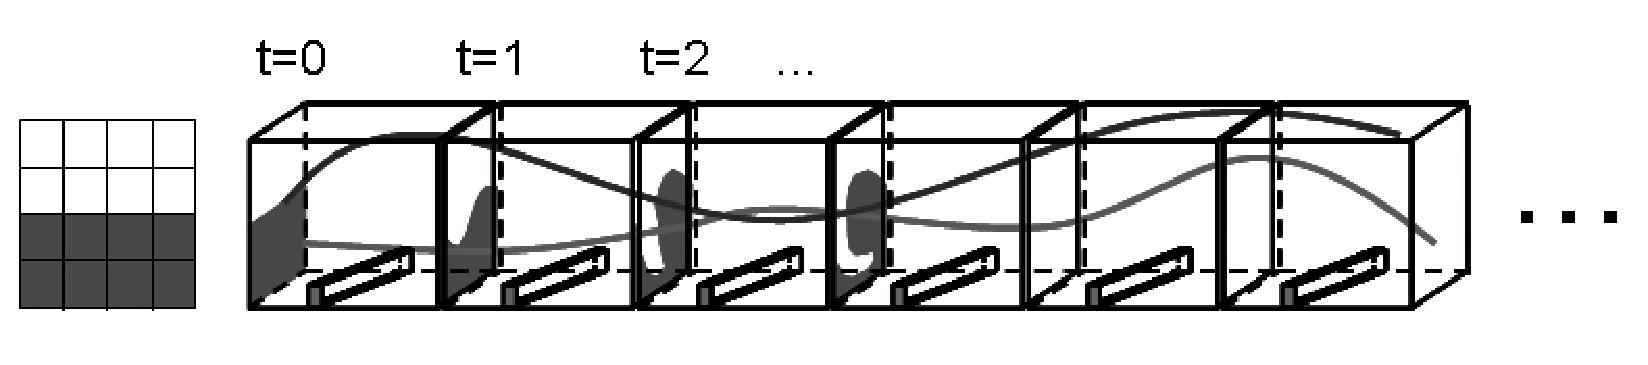
\includegraphics[width=0.8\textwidth,trim=1cm 1cm 0cm 0cm]{mixingchannel}}

\centerline{\includegraphics[width=0.8\textwidth,trim=1cm 1cm 0cm 0cm]{aaa}}
%%%%%%%%%%%%%%%%%%%%%%%%%%%%%%%%%%%%%%%%%%%%%%%%%%%%%%%%%%%%%%%%%%%%%%%%%
%%%%%%%%%%%%%%%%%%%%%%%%%%%%%%%%%%%%%%%%%%%%%%%%%%%%%%%%%%%%%%%%%%%%%%%%%
\newpage
\oursection{Stokes Equation and Darcey Flow}

\begin{itemize}
\item Generalized Stokes partial differential equation for imcompressible flow (Darcey equation)
       \begin{eqnarray*}
       ( -\mu\triangle + \mathbf{\alpha} \mathbf{I}) \mathbf{u} +\nabla  \mathbf{p} & = & \mathbf{f}\\
       \mbox{div} \mathbf{u}& = & 0 
       \end{eqnarray*}

       $\mathbf{u}$: velocity, $\mathbf{p}$: pressure, $\mathbf{f}$: body force and boundary conditions 
       $\mu$: viscosity, and $\bf{\alpha}$: inverse permeability 
\item Discrete version 
       \begin{equation}
       \left[\begin{matrix}
       -\mu \mathbf{L} + \mathbf{H} \mathbf{\bar{\alpha}}  & \mathbf{G}\\
       \mathbf{D}               &  0 
       \end{matrix} \right]
	\left[\begin{matrix}
  	\mathbf{\bar{u}} \\ \mathbf{\bar{p}}
	\end{matrix} \right]= 
	\left[\begin{matrix}
  	\mathbf{\bar{f}} \\ \mathbf{0}
	\end{matrix} \right]
	\end{equation}
\end{itemize}

%%%%%%%%%%%%%%%%%%%%%%%%%%%%%%%%%%%%%%%%%%%%%%%%%%%%%%%%%%%%%%%%%%%%%%%%%
%%%%%%%%%%%%%%%%%%%%%%%%%%%%%%%%%%%%%%%%%%%%%%%%%%%%%%%%%%%%%%%%%%%%%%%%%
\newpage
\oursection{Forming the optimization problem}

\begin{eqnarray*}
  \mbox{minimize} & g(\mathbf{\bar{u}},\mathbf{\bar{p}},\mathbf{\bar{\alpha}}) \\
  \mbox{s.t.}&  
	\left[\begin{matrix}
 	 -\mu \mathbf{L} + \mathbf{H} \mathbf{\bar{\alpha}}  & \mathbf{G}\\
 	  \mathbf{D}               &  0 
	\end{matrix} \right]
	\left[\begin{matrix}
	  \mathbf{\bar{u}} \\ \mathbf{\bar{p}}
	\end{matrix} \right]= 
	\left[\begin{matrix}
 	 \mathbf{\bar{f}} \\ \mathbf{0}
	\end{matrix} \right] \\
  & \mathbf{0}\le \mathbf{\bar{\alpha}} \le \alpha_M\mathbf{1}  
\end{eqnarray*}

The Objective Functions: 
\begin{itemize}
\setlength{\topsep}{0cm}\setlength{\parskip}{0cm}\setlength{\parsep}{0cm}\setlength{\itemsep}{0cm}
\item Linear functions on velocity
\item Maps between inlet and outlet
\item The second largest eigenvalue modulus of a Markov matrix 
\end{itemize}

%%%%%%%%%%%%%%%%%%%%%%%%%%%%%%%%%%%%%%%%%%%%%%%%%%%%%%%%%%%%%%%%%%%%%%%%%
%%%%%%%%%%%%%%%%%%%%%%%%%%%%%%%%%%%%%%%%%%%%%%%%%%%%%%%%%%%%%%%%%%%%%%%%%
\newpage
\oursection{The Map Defined by Streamlines}
\begin{tabular}{rl}
\includegraphics[width=0.5\textwidth,trim=1cm 1cm 0cm 0cm]{computedmixingchannel}&
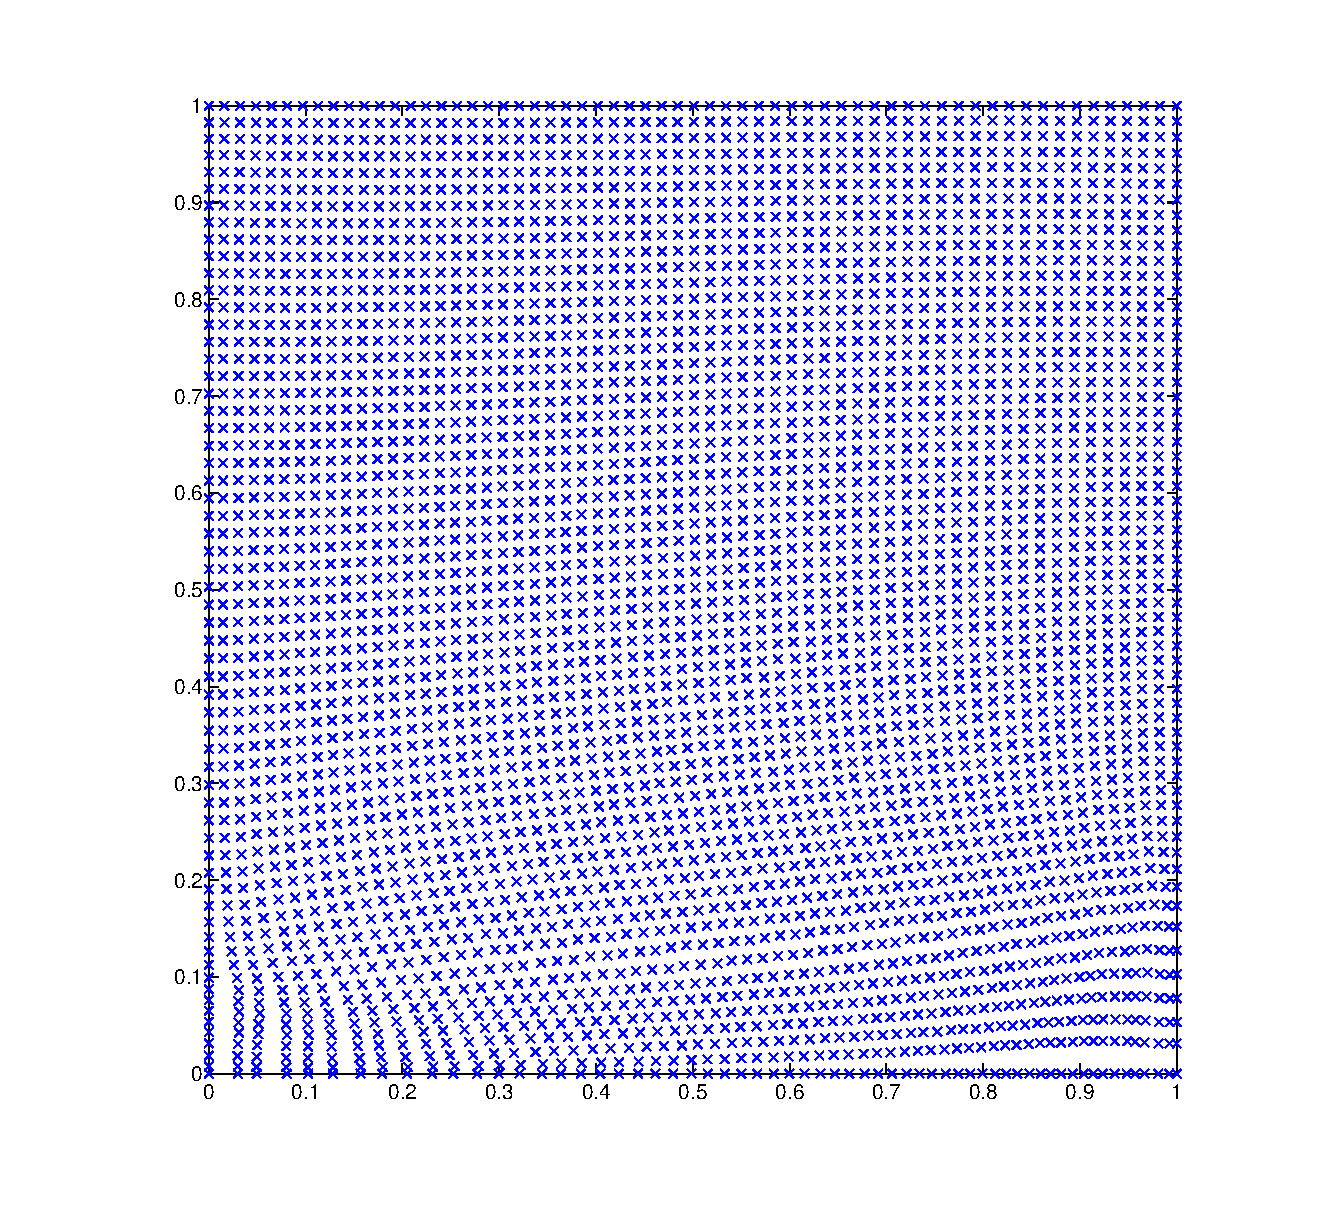
\includegraphics[width=0.5\textwidth,trim=1cm 1cm 0cm 0cm]{mappedpoints}
\end{tabular}

%%%%%%%%%%%%%%%%%%%%%%%%%%%%%%%%%%%%%%%%%%%%%%%%%%%%%%%%%%%%%%%%%%%%%%%%%
\newpage
\oursection{The Objective Function}


%%%%%%%%%%%%%%%%%%%%%%%%%%%%%%%%%%%%%%%%%%%%%%%%%%%%%%%%%%%%%%%%%%%%%%%%%
%%%%%%%%%%%%%%%%%%%%%%%%%%%%%%%%%%%%%%%%%%%%%%%%%%%%%%%%%%%%%%%%%%%%%%%%%
\newpage
\oursection{Finding a decent direction}
Chain rule : $\frac{d\lambda}{d\alpha} = \frac{d\lambda}{dA}\frac{dA}{dv}\frac{dv}{d\alpha}$
\begin{itemize}
\item $\frac{d\lambda}{dA}$ : Eigenvector  
\item $\frac{dA}{dv}\frac{dv}{d\alpha}$ : Adjoint method
\item $\frac{dv}{d\alpha}$ : Streamline
\end{itemize}


%%%%%%%%%%%%%%%%%%%%%%%%%%%%%%%%%%%%%%%%%%%%%%%%%%%%%%%%%%%%%%%%%%%%%%%%%




%%%%%%%%%%%%%%%%%%%%%%%%%%%%%%%%%%%%%%%%%%%%%%%%%%%%%%%%%%%%%%%%%%%%%%%%%
%%%%%%%%%%%%%%%%%%%%%%%%%%%%%%%%%%%%%%%%%%%%%%%%%%%%%%%%%%%%%%%%%%%%%%%%%
\newpage
\oursection{Tools and solving}
%%%%%%%%%%%%%%%%%%%%%%%%%%%%%%%%%%%%%%%%%%%%%%%%%%%%%%%%%%%%%%%%%%%%%%%%%
\begin{itemize}
\item Parallel linear equation solver PETSC
\item Eigenvector and eigenvalues :SLEPC
\item Develope a package that communicates PETSC and Matlab 
\end{itemize}

%%%%%%%%%%%%%%%%%%%%%%%%%%%%%%%%%%%%%%%%%%%%%%%%%%%%%%%%%%%%%%%%%%%%%%%%%
\newpage
\oursection{Results}





%%%%%%%%%%%%%%%%%%%%%%%%%%%%%%%%%%%%%%%%%%%%%%%%%%%%%%%%%%%%%%%%%%%%%%%%%
%%%%%%%%%%%%%%%%%%%%%%%%%%%%%%%%%%%%%%%%%%%%%%%%%%%%%%%%%%%%%%%%%%%%%%%%%
%%%%%%%%%%%%%                 TOPIC b                          %%%%%%%%%%
%%%%%%%%%%%%%%%%%%%%%%%%%%%%%%%%%%%%%%%%%%%%%%%%%%%%%%%%%%%%%%%%%%%%%%%%%
%%%%%%%%%%%%%%%%%%%%%%%%%%%%%%%%%%%%%%%%%%%%%%%%%%%%%%%%%%%%%%%%%%%%%%%%%
\newpage
\oursection{\mytopicb}



%%%%%%%%%%%%%%%%%%%%%%%%%%%%%%%%%%%%%%%%%%%%%%%%%%%%%%%%%%%%%%%%%%%%%%%%%
\newpage
\oursection{Mixing Trajectories}
%%%%%%%%%%%%%%%%%%%%%%%%%%%%%%%%%%%%%%%%%%%%%%%%%%%%%%%%%%%%%%%%%%%%%%%%%





%%%%%%%%%%%%%%%%%%%%%%%%%%%%%%%%%%%%%%%%%%%%%%%%%%%%%%%%%%%%%%%%%%%%%%%%%
%%%%%%%%%%%%%%%%%%%%%%%%%%%%%%%%%%%%%%%%%%%%%%%%%%%%%%%%%%%%%%%%%%%%%%%%%
%%%%%%%%%%%%%                 TOPIC c                          %%%%%%%%%%
%%%%%%%%%%%%%%%%%%%%%%%%%%%%%%%%%%%%%%%%%%%%%%%%%%%%%%%%%%%%%%%%%%%%%%%%%
%%%%%%%%%%%%%%%%%%%%%%%%%%%%%%%%%%%%%%%%%%%%%%%%%%%%%%%%%%%%%%%%%%%%%%%%%
\newpage
\oursection{\mytopicc}
   \begin{itemize}
      \item Cutoff phenomenon of Random Walks on Finite Groups
      \item Symbolic Dynamics and Sthochastic Symbolic Dynamics
      \item Chaos and Cutoff Phenomenon
   \end{itemize}

%%%%%%%%%%%%%%%%%%%%%%%%%%%%%%%%%%%%%%%%%%%%%%%%%%%%%%%%%%%%%%%%%%%%%%%%%
\newpage
\oursection{Chaotic Map Simulations}


%%%%%%%%%%%%%%%%%%%%%%%%%%%%%%%%%%%%%%%%%%%%%%%%%%%%%%%%%%%%%%%%%%%%%%%%%
%%%%%%%%%%%%%%%%%%%%%%%%%%%%%%%%%%%%%%%%%%%%%%%%%%%%%%%%%%%%%%%%%%%%%%%%%
\newpage
\oursection{Cutoff phenomenon of Random Walks on Finite Groups}
%%%%%%%%%%%%%%%%%%%%%%%%%%%%%%%%%%%%%%%%%%%%%%%%%%%%%%%%%%%%%%%%%%%%%%%%%


%%%%%%%%%%%%%%%%%%%%%%%%%%%%%%%%%%%%%%%%%%%%%%%%%%%%%%%%%%%%%%%%%%%%%%%%%
%%%%%%%%%%%%%%%%%%%%%%%%%%%%%%%%%%%%%%%%%%%%%%%%%%%%%%%%%%%%%%%%%%%%%%%%%
\newpage
\oursection{Symbolic Dynamics and Sthochastic Symbolic Dynamics}
%%%%%%%%%%%%%%%%%%%%%%%%%%%%%%%%%%%%%%%%%%%%%%%%%%%%%%%%%%%%%%%%%%%%%%%%%


%%%%%%%%%%%%%%%%%%%%%%%%%%%%%%%%%%%%%%%%%%%%%%%%%%%%%%%%%%%%%%%%%%%%%%%%%
%%%%%%%%%%%%%%%%%%%%%%%%%%%%%%%%%%%%%%%%%%%%%%%%%%%%%%%%%%%%%%%%%%%%%%%%%
\newpage
\oursection{Chaos and Cutoff Phenomenon}
%%%%%%%%%%%%%%%%%%%%%%%%%%%%%%%%%%%%%%%%%%%%%%%%%%%%%%%%%%%%%%%%%%%%%%%%%





%%%%%%%%%%%%%%%%%%%%%%%%%%%%%%%%%%%%%%%%%%%%%%%%%%%%%%%%%%%%%%%%%%%%%%%%%
%%%%%%%%%%%%%%%%%%%%%%%%%%%%%%%%%%%%%%%%%%%%%%%%%%%%%%%%%%%%%%%%%%%%%%%%%
\newpage
\oursection{Conclusion}

%%%%%%%%%%%%%%%%%%%%%%%%%%%%%%%%%%%%%%%%%%%%%%%%%%%%%%%%%%%%%%%%%%%%%%%%%%
\end{document}
